\begin{tikzpicture}
\path[mindmap,
    text = white,
    every node/.style = {
      concept,
      circular drop shadow
    },
    root/.style = {
      concept color = red!40,
      font = \Large\bfseries, 
      text width = 8em
    },
    level 1 concept/.append style = {
      concept color = blue!40,
      font = \Large\bfseries,
      sibling angle = 150,
      text width = 8em,
      level distance = 15em,
      inner sep = 0pt
    },
    level 2 concept/.append style = {
      concept color = teal!20,
      font = \bfseries,
      sibling angle = 20,
      level distance = 9em
    },
  ]
  node[root] {Set \\ Theory} [counterclockwise from = 195]
    child[] {
      node {A Branch of Mathematics} [clockwise from = -90]
	% child [] {node (cantor) [] {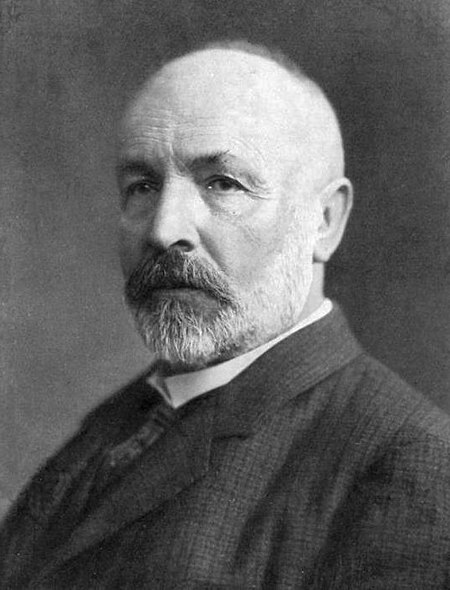
\includegraphics[scale = 0.60]{figs/Cantor}}}
    }
    child[] {
      node {Foundation of Mathematics \\ {\small (+ Logic)}} [counterclockwise from = 195]
	% child [] {node (frege) [] {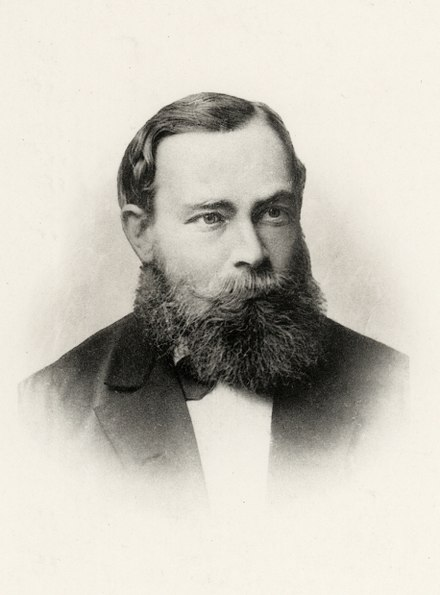
\includegraphics[scale = 0.30]{figs/Frege}}}
	% child [] {node (russell) [] {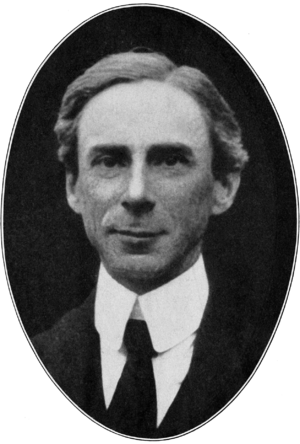
\includegraphics[scale = 0.30]{figs/Russell}}}
	% child [] {node (zermelo) [] {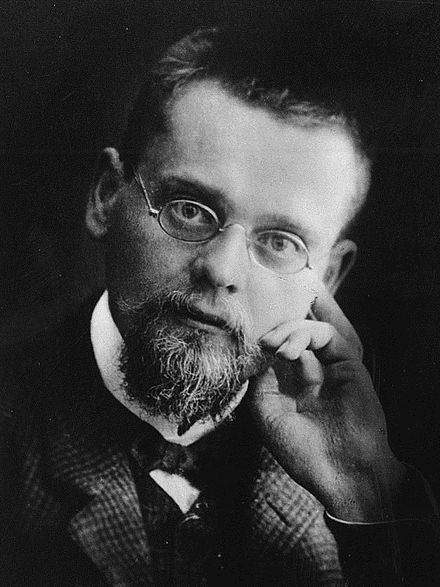
\includegraphics[scale = 0.30]{figs/Zermelo}}}
	% child [] {node (von) [] {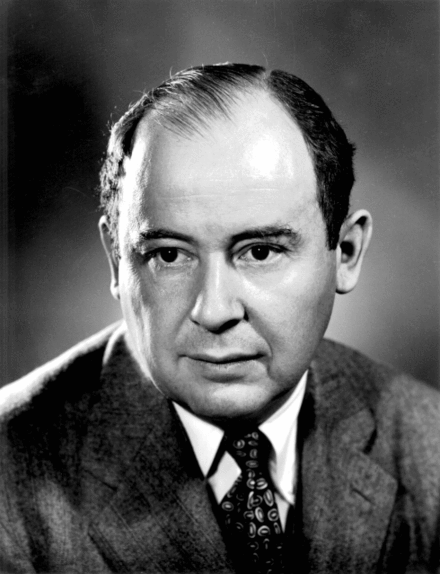
\includegraphics[scale = 0.30]{figs/von-Neumann}}}
    };
\end{tikzpicture}